\chapter{Filter Design}
\label{app:filterdesign}

Filtering the recorded signal can be useful to isolate certain frequencies of the signal as well as unmasking source with different frequency content or different levels. The min-power SRP-PHAT algorithm use the PHAT transform, which whiten the magnitude of the signal in order to only use the phase information to localize. For this reason a zero-phase filter is considered in our specific case where causality is not an issue but a linear-phase filter could also be used. The low pass and high pass filter are design using Matlab Filter Designer. Design specification of the low pass is $fs = 131072 Hz$, minimum order, FIR equiripple, stop band $80dB$, stop band frequency $300Hz$ and pass band frequency $100Hz$. The filter order is 1659. Figure \ref{fig:filterlowpass300} and \ref{fig:filterhighpass300} shows the frequency and impulse response of each filters.

\begin{figure}[H]
    \centering
\vskip \baselineskip
\begin{subfigure}[b]{0.96\textwidth}
    \centering
    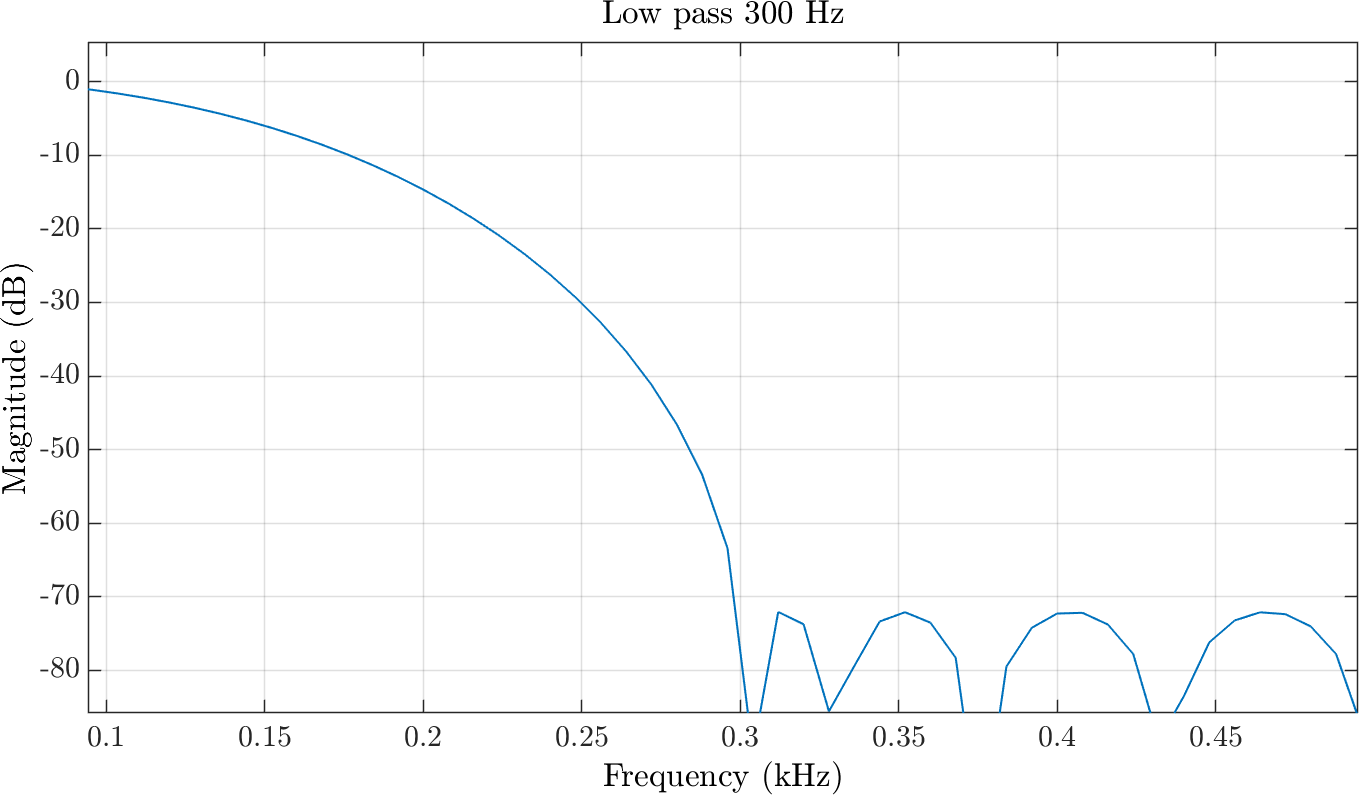
\includegraphics[width=0.9\textwidth]{Figures/lowpass300zommed.png}
\end{subfigure}
\vskip \baselineskip
\begin{subfigure}[b]{0.96\textwidth}
    \centering
    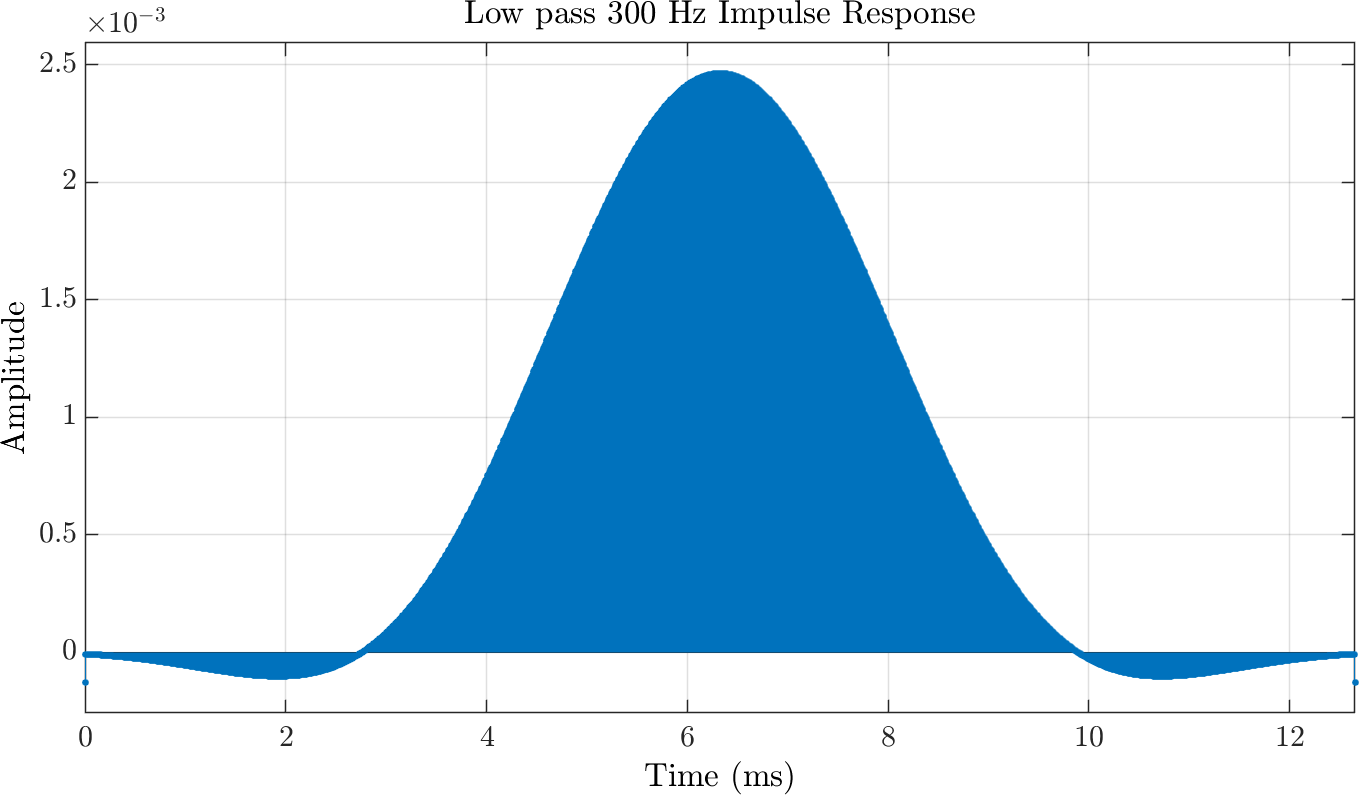
\includegraphics[width=0.9\textwidth]{Figures/lowpass300IR.png}
\end{subfigure}
\caption{Figures depict the frequency response and impulse response of the 300Hz low pass filter}
\label{fig:filterlowpass300}
\end{figure}

Design specification of the High pass is $fs = 131072 Hz$, minimum order, FIR equiripple, stop band $80dB$, stop band frequency $100Hz$ and pass band frequency $300Hz$. The filter order is 1801.
\begin{figure}[H]
    \centering
\vskip \baselineskip
\begin{subfigure}[b]{0.96\textwidth}
    \centering
    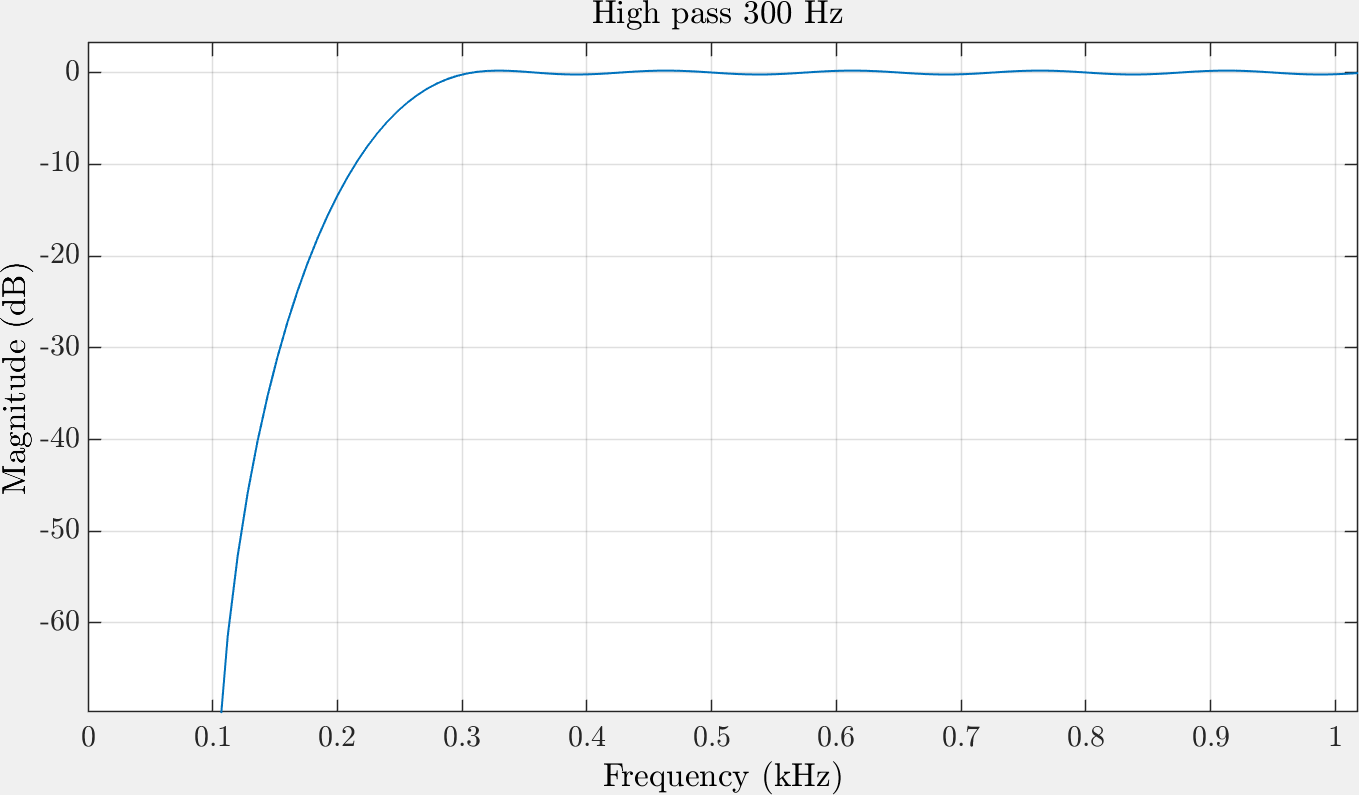
\includegraphics[width=0.9\textwidth]{Figures/highpass300zoomed.png}
\end{subfigure}
\vskip \baselineskip
\begin{subfigure}[b]{0.96\textwidth}
    \centering
    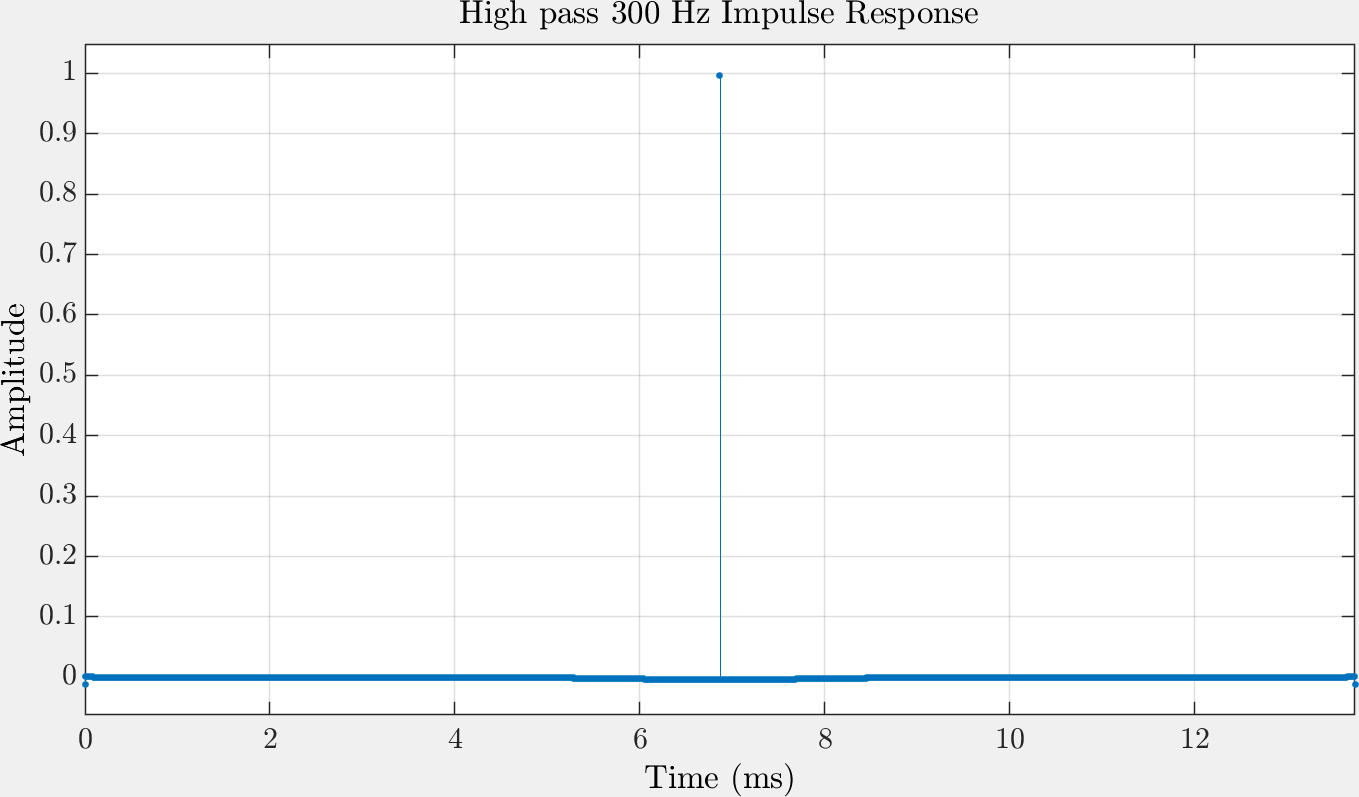
\includegraphics[width=0.9\textwidth]{Figures/highpass300IR.png}
\end{subfigure}
\caption{Figures depict the frequency response and impulse response of the 300Hz High pass filter}
\label{fig:filterhighpass300}
\end{figure}

In order to zero-phase filter the signal, the signal are filter once, then inverted and filer again. Matlab function filtfilt is used.